\documentclass[a4paper,11pt]{article}

%% Page format
\usepackage[headheight=110pt,hscale=0.75,vscale=0.8,centering]{geometry}
\usepackage{fancyhdr}
\pagestyle{fancy}
\fancyhf{}
\renewcommand{\headrulewidth}{0.4pt}
\renewcommand{\footrulewidth}{0.4pt}
\lhead{Impacts of transmission switching in zonal electricity markets}
\rhead{}
\rfoot{\thepage}
\fancypagestyle{plain}{
	\fancyhf{}
	\rfoot{\thepage}
	\renewcommand{\headrulewidth}{0pt}	
}

%% Packages for graphics and figures
\usepackage{graphicx}
\usepackage{xcolor}
\definecolor{darkgreen}{rgb}{0,0.5,0}
\usepackage[font={color=blue}]{caption}

\usepackage{tikz}
\usetikzlibrary{positioning}
\usetikzlibrary{shapes,arrows}
\usetikzlibrary{trees}
\usepackage{xkcdcolors}

%% Packages for equations
\usepackage{amsthm}
\usepackage{amsfonts}
\usepackage{amsmath}
\usepackage{amssymb}
\usepackage{bbm}
\usepackage{eurosym}

%% Tables
\usepackage{multirow}

%% Hyperlinks
\usepackage{hyperref}

%% Lists
\usepackage{enumitem}

%% Tikz
\usepackage{tikz}
\usetikzlibrary{positioning, arrows.meta}
\usepackage{pgfplotstable}
\pgfplotsset{compat=1.12}
\newcommand{\keepred}[1]{{\leavevmode\color{red}{#1}}}

%% Here
\usepackage{here}

%% Units
\usepackage{siunitx}

%% Custom commands
\newcommand{\st}{\mathrm{s.t.}~}
\newcommand{\argmin}{\mathrm{arg\,min}}
\newcommand{\argmax}{\mathrm{arg\,max}}
\newcommand{\quoted}[1]{``#1''}
\newcommand{\proj}[2]{\mathrm{proj}_{#1}\left(#2\right)}
\newcommand{\conv}[1]{\mathrm{conv}\left(#1\right)}
\newcommand{\resp}[1]{
	\begin{quote}
		\color{blue}
		#1
	\end{quote}}
\newcommand{\modification}[1]{
	\begin{quote}
		\itshape
		\color{red}
		#1
	\end{quote}}
\renewcommand{\thetable}{A\arabic{table}}

\newtheorem{theorem}{Theorem}

% title on the first page
\title{Impacts of Transmission Switching in Zonal Electricity Markets - Part II \\[.25cm]
	\Large{Responses to Reviewer Observations - Round 2}}
\author{Quentin Lété, \texttt{quentin.lete@uclouvain.be} \\
	Anthony Papavasiliou, \texttt{anthony.papavasiliou@uclouvain.be}}
\date{\today}

% short title -- to be shown at the top right of every page
\rhead{}

\newcommand{\anthony}[1]{{\leavevmode\color{xkcdOrange}{#1}}}
% \newcommand{\quentin}[1]{{\leavevmode\color{xkcdGreen}{#1}}}
% \newcommand{\anthony}[1]{#1}
\newcommand{\quentin}[1]{#1}

\begin{document}
\maketitle

\section*{Organization}

This document develops our responses to the observations and comments raised by the reviewers of our original manuscript ``Impacts of Transmission Switching in Zonal Electricity Markets - Part II'' in the secound round. The document also explains modifications to the manuscript that were inspired by the comments of the reviewers.

The document is organized into 2 sections, each of which corresponds to a different reviewer. We present reviewers' comments in black font and our responses using indented \textcolor{blue}{blue} paragraphs. Modifications to the manuscript are highlighted in \textcolor{blue}{blue} and, occasionally, repeated for convenience in the present document in indented italic \textcolor{red}{red} paragraphs.

\section{Reviewer \#1:}
My comments from Part II echo my concerns from Part I. They are only briefly described below.

\resp{
    We address the reviewer's comment about unit commitment in the response letter to Part I. 
}

\begin{enumerate}
    \item The paper appears to contradict itself on whether the day-ahead model includes unit commitment or not.
\end{enumerate}

\resp{
    The model includes unit commitment. We provide a detailed discussion about the role of unit commitment in our paper in our response letter to the first part of the paper.
}

\begin{enumerate}
    \setcounter{enumi}{1}
    \item Do the theoretical results of Part I hold if unit commitment is included in the day-ahead model?
\end{enumerate}

\resp{
    Our zonal day-ahead model includes unit commitment. 
    The reviewer is referred to the response letter of Part I for a detailed discussion on how we changed the motivation of the paper in order to avoid any ambiguity about whether our paper includes unit commitment.
}

\begin{enumerate}
    \setcounter{enumi}{2}
    \item The authors do not clearly describe how prices are generated in their ``zonal day-ahead model."
\end{enumerate}

\resp{
    The goal of our paper is to quantify the inefficiencies of the European zonal design with respect to unit commitment and to measure the impact of switching on reducing these inefficiencies. 
    In order to measure these inefficiencies, the relevant output of the day-ahead model is the unit commitment decision and our model does not produce prices explicitly. 
    The assumption that is made in our model is that units are committed while maximizing the total welfare. 
    This is the result that is obtained with usual pricing mechanisms like IP pricing \cite{Oneill2004} and convex hull pricing \cite{Gribik2007}. 
    
    The question of the most appropriate pricing mechanism is an ongoing debate among European stakeholders.
    Traditionally, the European pricing rules have forbidden the recourse to uplift payments, at the cost of a potential loss in welfare \cite{MadaniThesis}.
    However, these rules are being reconsidered and there is an ongoing discussion with Nominated European Market Operators (NEMOs) about the consideration of so-called non-uniform pricing rules (i.e. welfare maximization supported by side payments) \cite{Epri_pres}.
    %the market is expected to evolve towards a full welfare maximization approach. 
    We do not address the question of the most appropriate pricing mechanism in the presence of non-convexities in our paper and, instead, assume that units are committed under welfare maximization. 
    This approach leads to a best-case investigation of zonal pricing and enables us to focus on the inefficiencies in unit commitment that result from the simplified representation of transmission constraints in a zonal day-ahead model. 
    
    Finally, we note that our model could in theory be extended to compute prices under the different pricing mechanisms. 
    In the case of IP pricing, the procedure would be simply to fix the switching and commitment variables in order to obtain a linear problem. 
    The dual variable of the zonal balance constraint produces the zonal price. 
    In the case of convex hull pricing, the methodology would be to fix the switching variables to their optimal value and obtain the zonal prices as the optimal values of the Lagrangian dual variables of the zonal balance constraint.
    In the case of the current European pricing rules that require strict linear prices, the prices could be obtained by again fixing the switching variables and following the approach presented in \cite{madani2015} in order to reformulate the equilibrium problem as a Mixed Integer Problem.
    A full analysis of the implications of our zonal day-ahead model on pricing is, however, outside the scope of the paper, and is the subject of follow-up research. 
    
    \quentin{Let us now illustrate on a small three-node two-zone example how the prices could be determined. 
    We use a similar instance as the one used in the response letter to part 1 with some slight changes in the data. 
    The instance with the data, inspired by the small example presented in \cite{Schiro2015}, is presented in Fig. \ref{fig:triangle}. 
    \begin{figure}
        \centering
        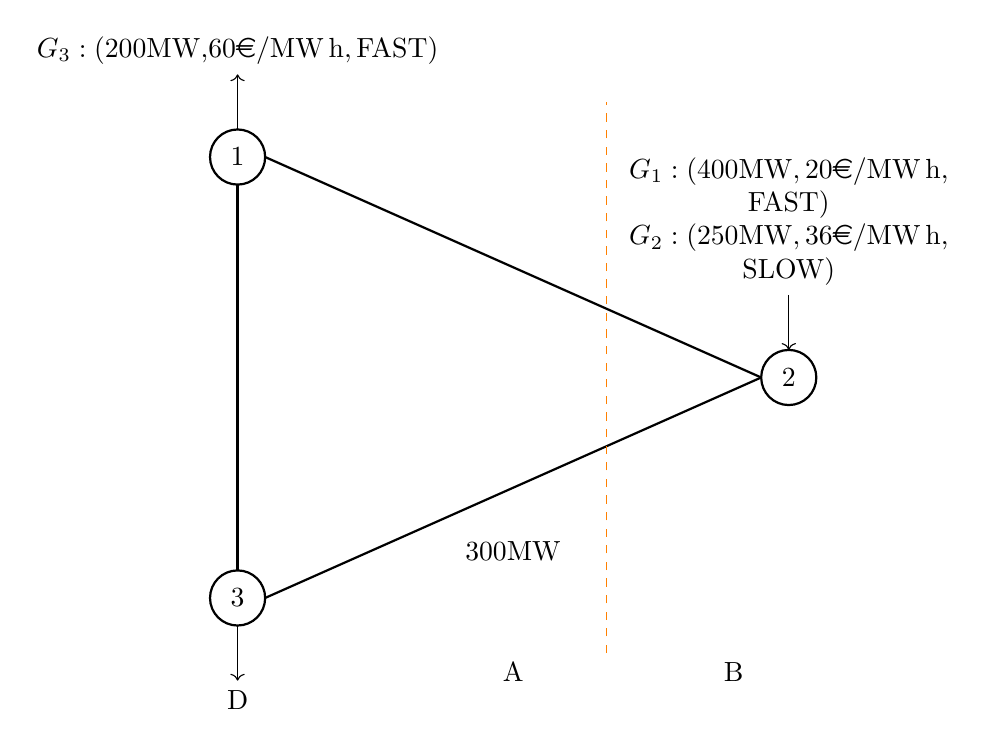
\begin{tikzpicture}[scale=7]
	\draw [thick] (0, 0.1) circle [radius=0.05];
	\draw [thick] (1, 0.5) circle [radius=0.05];
	\draw [thick] (0, 0.9) circle [radius=0.05];
	\node at (0, 0.1) {3};
	\node at(1, 0.5) {2};
	\node at (0, 0.9) {1};
    \draw [thick] (0.05, 0.9) -- (0.95, 0.5);
    \draw [thick] (0.05, 0.1) -- (0.95, 0.5);
	\draw [thick] (0, 0.15) -- (0, 0.85);
    % \node [right] at (-0.2, 0.5) {$50\si{\mega\watt}$};
    % \node [right] at (0.32, 0.85) {$200 \si{\mega\watt}$};

	\draw [->] (1, 0.65) -- (1, 0.55);
	\node [above, align=center] at (1, 0.65) {$G_1:(400\si{\mega\watt},20\text{\euro}/\si{\mega\watt\hour}$, \\ $\text{FAST})$ \\ $G_2:(250\si{\mega\watt},36\text{\euro}/\si{\mega\watt\hour}$, \\ $\text{SLOW})$};
	
% 	\draw [->] (1, 0.45) -- (1, 0.35);
% 	\node [below, align=center] at (1, 0.35) {$G_2:(100\si{\mega\watt},20\text{\euro}/\si{\mega\watt\hour}$, \\ $\text{SLOW})$}

	\draw [->] (0, 0.95) -- (0, 1.05);
	\node [above] at (0, 1.05) {$G_3:(200\si{\mega\watt}$, \\ $60\text{\euro}/\si{\mega\watt\hour}, \text{FAST})$};

%     \draw (-0.05, 0.9) -- (-0.15, 0.9);
%     \draw [->] (-0.15, 0.9) -- (-0.15, 0.8);
% 	\node [below] at (-0.15, 0.8) {$C:200\si{\mega\watt}$};

    \draw [->] (0, 0.05) -- (0, -0.05);
    \node [below] at (0, -0.05) {D};
    
    % \draw [->] (-0.15, 0.1) -- (-0.05, 0.1);
    % \draw (-0.15, 0.1) -- (-0.15, 0.2);
    % \node [above, align=center] at (-0.25, 0.2) {$G_3:(200\si{\mega\watt}$, \\ $60\text{\euro}/\si{\mega\watt\hour}$, FAST)};

	\node [above] at (0.5, 0.15) {$300 \si{\mega\watt}$};
	\node [below] at (0.5, 0) {A};
	\node [below] at (0.9, 0) {B};
	\draw [dashed, color=orange] (0.67, 0) -- (0.67, 1);
\end{tikzpicture}
        \caption{Three-node two-zone example for illustrating the different pricing mechanism.}
        \label{fig:triangle}
    \end{figure}
    In order to determine prices, the optimal switching decision will first be obtained by maximizing welfare. 
    Then, prices will be computed following the rules of each method with the fixed topology. The resulting prices for the different pricing methods discussed above are presented in table \ref{tab:my_label}.
    \begin{table}[H]
        \color{blue}
        \centering
        \begin{tabular}{c|c|c|c|c}
             Load level (D) & Lines switched & IP price & Convex hull price & EU-style price\footnotemark \\
             $\text{[MW]}$ & off &  [$\text{\euro}$/MWh] &  [$\text{\euro}$/MWh] &  [$\text{\euro}$/MWh] \\
             \hline
             300 & $\emptyset$ & 20 & 20 & 20 \\ 
             450 & $\emptyset$ & 60 & 36 & 60 \\
             550 & line 2-3 & 20 & 36 & 60 \\
             700 & line 2-3 & 60 & 60 & 60 \\
        \end{tabular}
        \caption{Switching decision and price in the different pricing mechanisms.}
        \label{tab:my_label}
    \end{table}}
    
    \footnotetext{{\color{blue}Note that the EU-style price leads to a different dispatch than IP and CHP pricing at a load level of 550MW, which translates to a loss of welfare. Generator $G_2$ is in that case not committed and is 'paradoxically rejected', which is allowed according to EU pricing rules. No side payments are required.}}
    
    Inspired by the comment of the reviewer, we have modified footnote n$^\circ$4 on page 3 of our original submission. % was probably misleading by suggesting that our model computes prices explicitly. 
    %Following the comment of the reviewer, we have modified this footnote. 
    We repeat this modification here for the convenient reference of the reviewer. 
    \begin{quotation}
        {\it
            We assume that the commitment is determined along with the topology \textcolor{red}{with the objective of maximizing welfare.
            Prices can be computed after the binary decisions have been fixed \cite{ONeill2010}. A full analysis of the implications of our zonal day-ahead model on pricing is however outside the scope of the paper, and is the subject of follow-up research.}
        }
    \end{quotation}
}

\section{Reviewer \#2:}
The authors addressed in a satisfactory way my prior major concern regarding the N-1 security rule. I have no further comment.

\resp{
    We thank the reviewer for the appreciation of our work.
}

\bibliographystyle{plain}
\bibliography{response}

\end{document}